\documentclass[11pt,a4paper]{report}
\usepackage[utf8]{inputenc}
\usepackage{amsmath}
\usepackage{amsfonts}
\usepackage{amssymb}
\usepackage{graphicx}
\usepackage[margin=1in]{geometry}  
\usepackage{caption}
\usepackage{subcaption}
\begin{document}

\chapter*{Assignment 5}
\section*{Task 1 - Optical Flow}

\subsection*{Observations}
Between the three cases, I noticed that the more spread out the two images are (i.e. the more frames that are missing between two compared frames), the longer the motion vectors are. This perhaps makes it easier to determine motion between images when the relative motion between frames is not high (i.e. high frame rate, low motion, very distant objects.) However, the LK method can be fairly prone to noise, giving false vectors. These could be mitigated by finding the fundamental matrix, as used in task 3, to reject outliers by RANSAC. 

\section*{Task 2 - Feature Matching}

\subsection*{Observations}

In this task, it is easy to see the problems that a blank wall or simple line can cause. For instance, many points on the edge of a straight line (i.e. the laptop) were matched incorrectly because they looked very similar. While the overall effect is correct, the outliers can cause a somewhat noticeable effect. However, using frames that are more distant in time can reduce this effect because the total distance moved can put many of the false matches out of the range of the search area. However, with blank or repetitive regions, the matches can result in false matches no matter what. The good matches, on the other hand, seem to be better matches overall.

Additionally, there is a tradeoff to be made with the size of the template relative to the search area. A larger template can ensure better matching, and a larger search area allows for a greater range of movement in the image. However, there is hit to processing time as either or both of these regions grow larger. When operating on several hundred points, this delay becomes noticeable. For general images, it seems that a small region for both of these is significant; however, in my debugging, I tested the chessboard images on this code and found that the highly repetitive image required a larger template and search field in order to give some degree of accuracy to the matches. I am as yet unsure how to mitigate this. 

\section*{Task 3 - Multi-Frame Tracking}

\begin{figure}[H]
\centering
\begin{subfigure}{.5\textwidth}
  \centering
  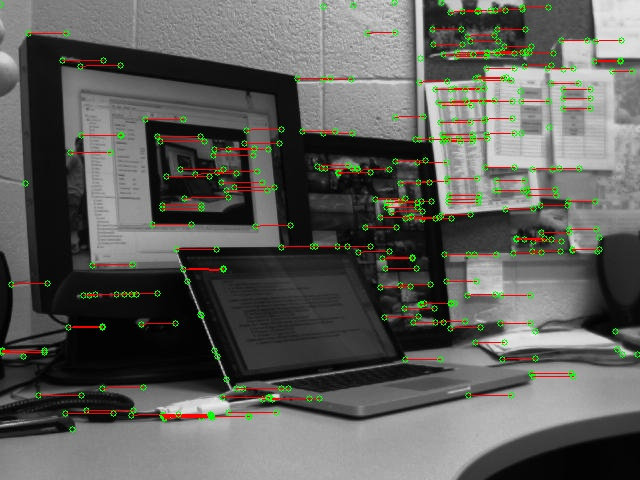
\includegraphics[height=4cm,keepaspectratio]{outParaRealStart}
  \caption{Start}
  \label{fig:sub1}
\end{subfigure}%
\begin{subfigure}{.5\textwidth}
  \centering
  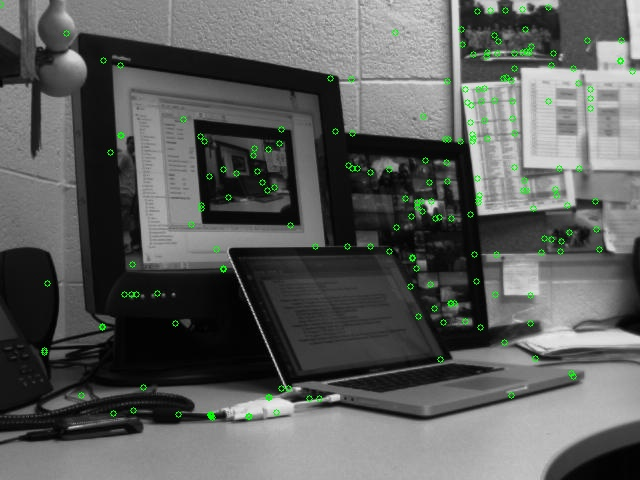
\includegraphics[height=4cm,keepaspectratio]{outParaRealEnd}
  \caption{End}
  \label{fig:sub2}
\end{subfigure}
\label{fig:test}
\caption{Parallel Real}
\end{figure}

\begin{figure}[H]
\centering
\begin{subfigure}{.5\textwidth}
  \centering
  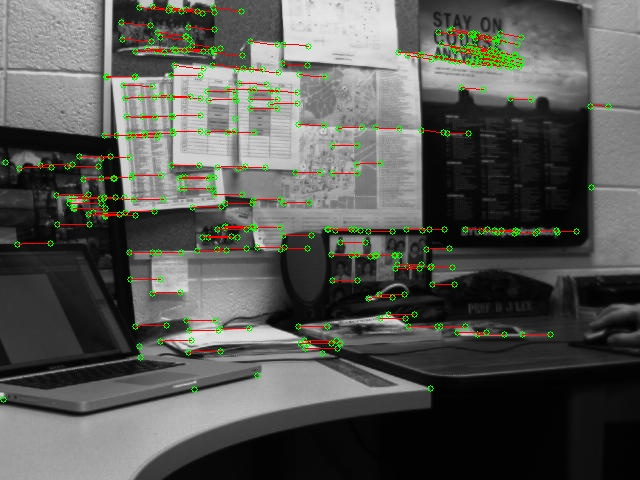
\includegraphics[height=4cm,keepaspectratio]{outTurnRealStart}
  \caption{Start}
  \label{fig:sub1}
\end{subfigure}%
\begin{subfigure}{.5\textwidth}
  \centering
  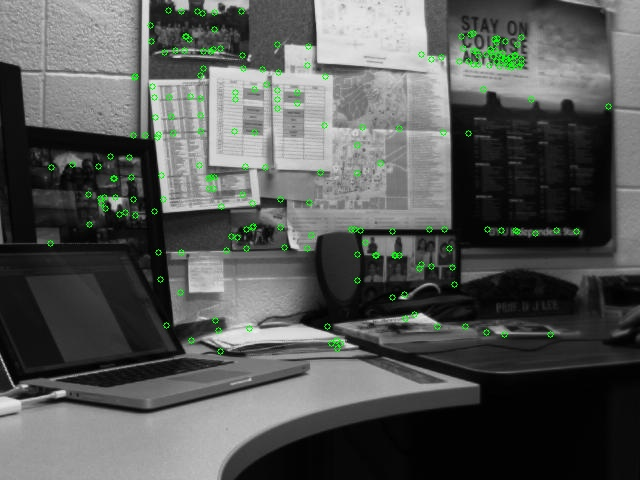
\includegraphics[height=4cm,keepaspectratio]{outTurnRealEnd}
  \caption{End}
  \label{fig:sub2}
\end{subfigure}
\label{fig:test}
\caption{Turn Real}
\end{figure}

\begin{figure}[H]
\centering
\begin{subfigure}{.5\textwidth}
  \centering
  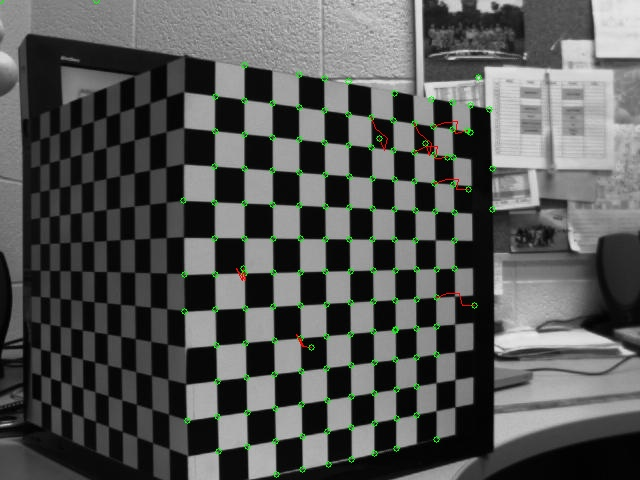
\includegraphics[height=4cm,keepaspectratio]{outParaCubeStart}
  \caption{Start}
  \label{fig:sub1}
\end{subfigure}%
\begin{subfigure}{.5\textwidth}
  \centering
  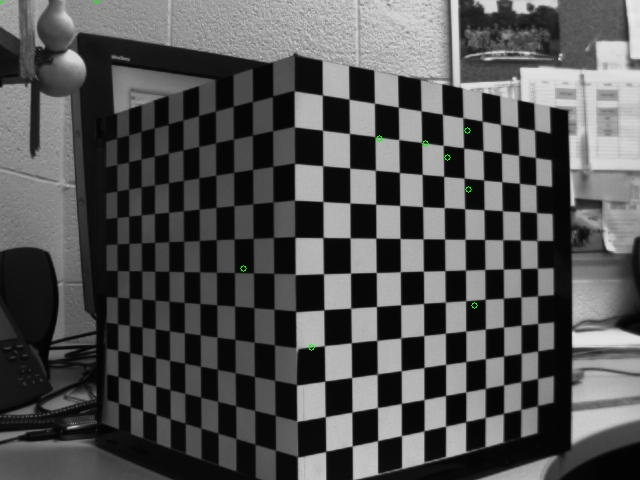
\includegraphics[height=4cm,keepaspectratio]{outParaCubeEnd}
  \caption{End}
  \label{fig:sub2}
\end{subfigure}
\label{fig:test}
\caption{Parallel Cube}
\end{figure}

\begin{figure}[H]
\centering
\begin{subfigure}{.5\textwidth}
  \centering
  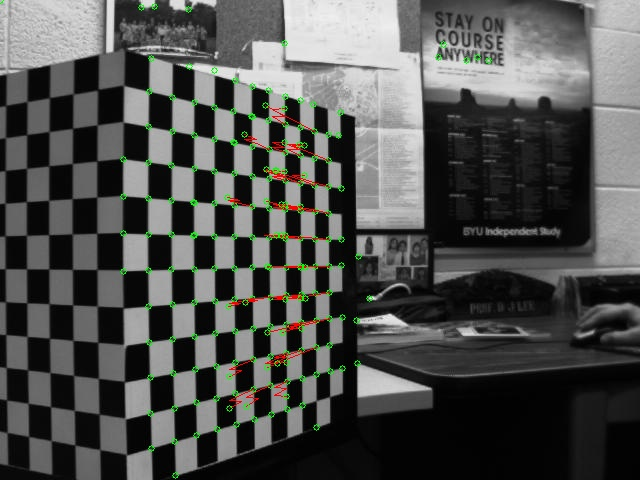
\includegraphics[height=4cm,keepaspectratio]{outTurnCubeStart}
  \caption{Start}
  \label{fig:sub1}
\end{subfigure}%
\begin{subfigure}{.5\textwidth}
  \centering
  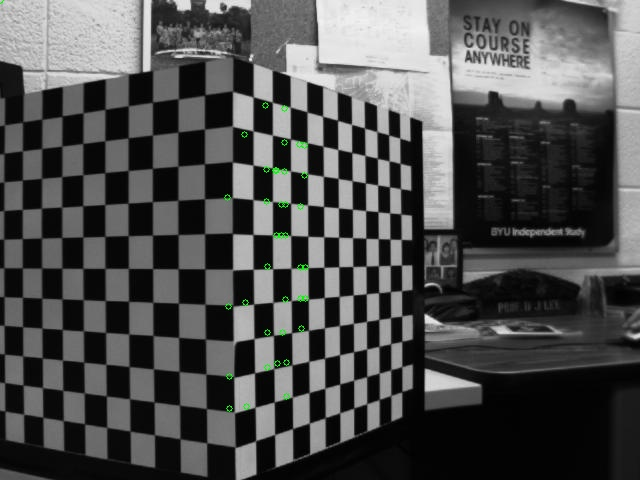
\includegraphics[height=4cm,keepaspectratio]{outTurnCubeEnd}
  \caption{End}
  \label{fig:sub2}
\end{subfigure}
\label{fig:test}
\caption{Turn Cube}
\end{figure}

\end{document}